\section{Tranformada LogOdds}

\subsection{Colinealidad}

\begin{wrapfigure}{r}{0.35\textwidth}
    \begin{center}
        \vspace{-1cm}
        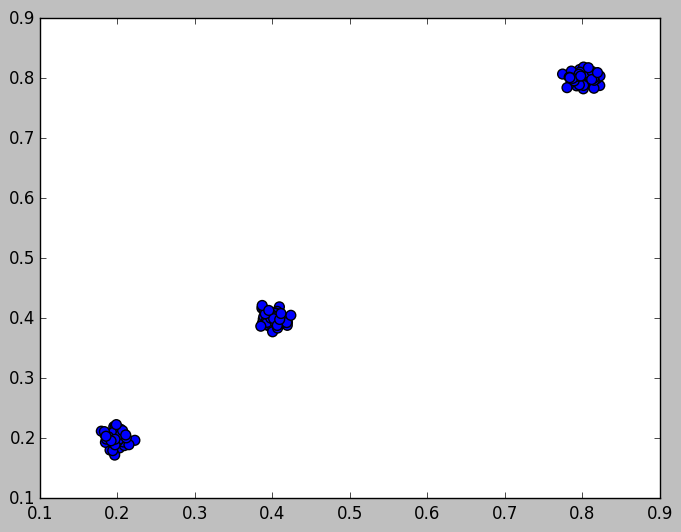
\includegraphics[width=0.35\textwidth]{img/3pop.png}
        \caption{Tres cluster colineales\-}
        \label{fig:3clusters}
    \end{center}
\end{wrapfigure} 

Cuando lo que se intentan agrupar vectores que son colineales usando como medida
de similitud la distancia coseno el resultado es aleatorio. Por ejemplo, cuando
se aplica el procedimiento sobre los puntos de la Figura \ref{fig:3clusters}
el resultado para Moreno es la Figura \ref{fig:3moreno}, mientras que el resultado
para LogOdds es el de la Figura \ref{fig:3logit}.\\

\vspace{1.5cm}

\begin{figure}[h!]
                                                                                                                        
\begin{minipage}[b]{\textwidth}
    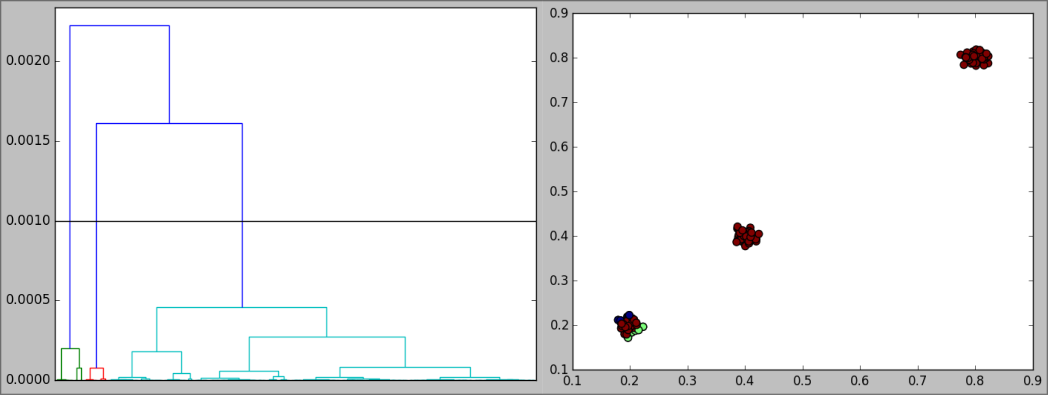
\includegraphics[width=\textwidth]{img/3pop_moreno.png}
    \caption{Clustering resultado de utilizar el m\'etodo Moreno}
    \label{fig:3moreno}
\end{minipage} ~

\end{figure}  

\begin{figure}[h!]
                                                                                                                        
\begin{minipage}[b]{\textwidth}
    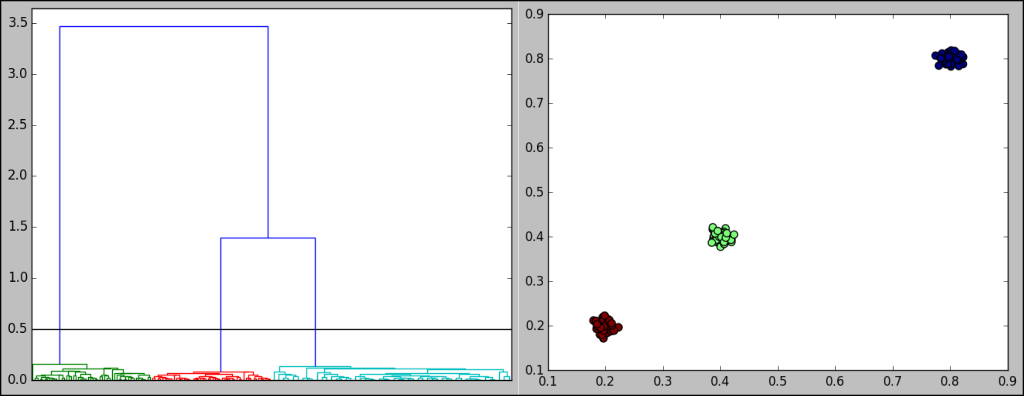
\includegraphics[width=\textwidth]{img/3pop_logit.png}
    \caption{Clustering resultado de utilizar el m\'etodo logit}
    \label{fig:3logit}
\end{minipage} ~

\end{figure}  


\subsection{Similitud vs Linkage}

La Figura \ref{fig:cos_cen} muestra cuatro vectores, sus posiciones en coordenadas
polares son: 

$$ p_1 = (0.4, 45^\circ);  p_2 = (0.3, 25^\circ); p_3 = (0.4, 66^\circ); p_4 = (0.4, 4.5^\circ)$$

Podemos apreciar que al principio $d(p_2,p_3) < d(p_3,p_4) < d(p_1,p_2)$, siendo
$d(x,y)$ la distancia coseno. Sin embargo, luego de utilizar el 
\textit{linkage centroid} sucede que $d(p_1,p_c) < d(p_4,p_c)$, esto es, $p_4$
es ahora el punto que mas lejos est\'a del centroide. Si crearamos el representante
del nuevo cluster usando el \'angulo medio entre $p_2$ y $p_3$, entonces $p_4$
seguir\'ia siendo el punto mas cercano a la uni\'on. \\

\begin{figure}[h!]
                                                                                                                        
\begin{minipage}[b]{\textwidth}
    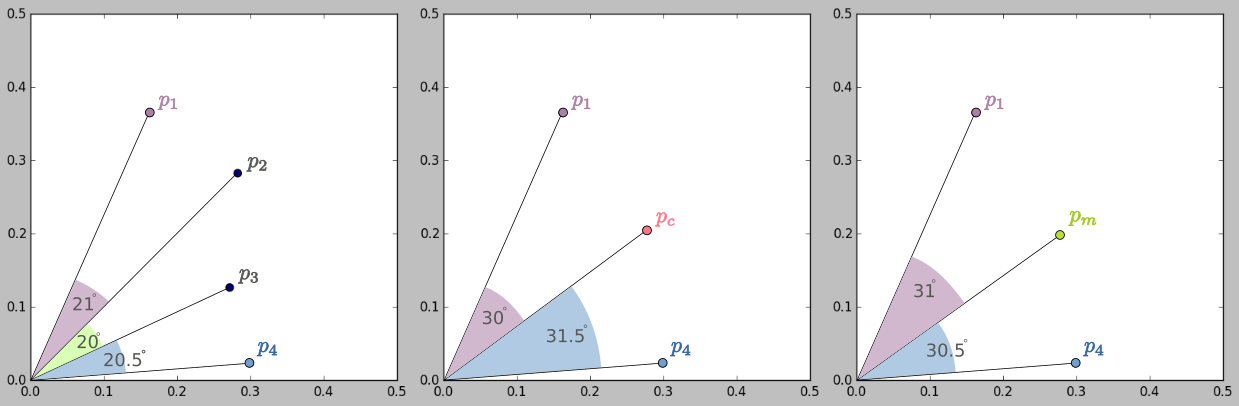
\includegraphics[width=\textwidth]{img/cosine_centroid.png}
    \caption{Contraejemplo para linkage centroide con la distancia coseno}
    \label{fig:cos_cen}
\end{minipage} ~

\end{figure}  

\textbf{Esto sucede tambi\'en con la distancia euclidea en logit}. En la Figura
\ref{fig:euc_cen}, para $l>2$, se cumple que $p_1$ est\'a m\'as cerca del centroide
que $p_4$. Recordemos que los valores dentro de los vectores luego de ser 
transformados usando LogOdds dejan de est\'ar acotados.

\begin{figure}[h!]
                                                                                                                        
\begin{minipage}[b]{\textwidth}
    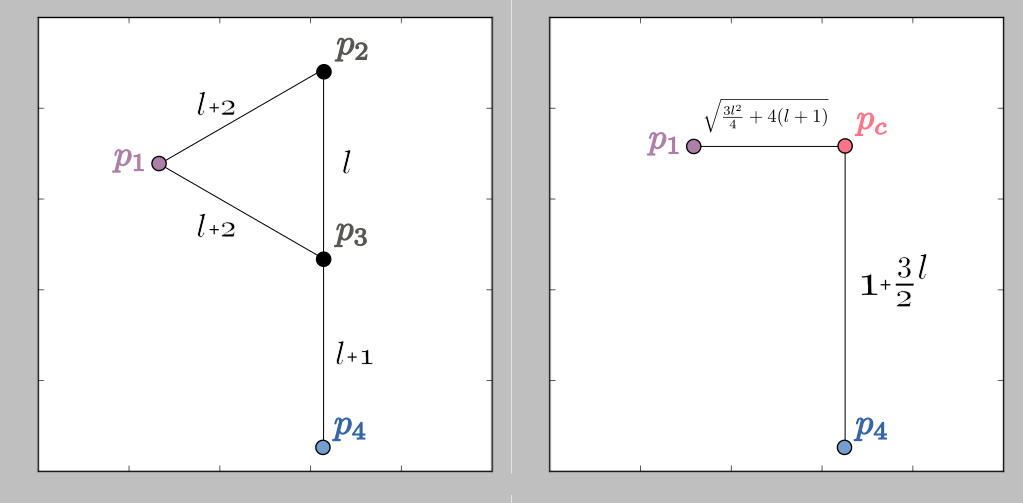
\includegraphics[width=\textwidth]{img/euclidean_centroid.png}
    \caption{Contraejemplo para linkage centroide con la distancia euclidea 
             luego de aplicar logit}
    \label{fig:euc_cen}
\end{minipage} ~

\end{figure}  

\subsection{Complejidad algor\'itmica}

Como ya explicamos, por cada iteraci\'on del algoritmo 
\textit{Agglomerative Herarchical Clustering} es necesario calcular un 
representante de la uni\'on y luego computar su distancia al resto. Sin embargo, 
al usar la m\'etrica euclideana junto con el \textit{linkage} centroide es posible
simplificar este paso. La formula de Lance y Williams permite computar las nuevas
distancias sin comparar explicitamente los clusters. Esto baja la complejidad
un orden de magnitud.


